\section{openHAB}
\label{sec:openhab} 
    Neben der erläuterten Home Assistant Plattform zählt openHAB zu den bekanntesten Open-Source-Systemen im 
    Bereich des \acs{SH}. Der \ac{OPENHAB} ist eine Plattform, bei der es sich um eine 
    Softwarelösung handelt, die auf Basis der Programmiersprache Java aufgebaut ist. Die Software steht unter 
    der Eclipse Public License und zählt zu der Rubrik der Open-Source-Software. Durch die Verwendung 
    von Java ist die Anwendung betriebssystemunabhängig und kann auf beliebigen Betriebssystemen laufen. 
    Ähnlich zu der vorgestellten Home Assistant Software bietet \acs{OPENHAB} ebenso Benutzeroberflächen, sog. User Interfaces, die durch 
    den Webbrowser, Android- und iOS-Geräte unterstützt werden. 
    \\
    \linebreak
    In Kombination mit Java wird bei \acs{OPENHAB} das \ac{OSGI}-Framework für die Modularität der Software verwendet. Mit Apache 
    Karaf wird ein Container bereitgestellt, der mit Eclipse Equinox als \acs{OSGI} Laufzeitumgebung agiert. Als 
    \acs{HTTP}-Server ist Jetty in Gebrauch. Die einzelnen Frameworks werden nicht im Detail erläutert, lediglich die für das 
    Verständnis des Konzeptes notwendigen.
    \\
    \linebreak
    Mit \acs{OPENHAB} wird eine hochmodulare Software zur Verfügung gestellt, die durch sogenannte \textit{Add-ons} erweitert 
    werden kann. Durch diese wird der Plattform eine breite Palette an Funktionen geboten. Physische Geräte können in 
    großer Anzahl mit der Plattform interagieren und verknüpft werden.\footnote{Einleitung zu openHAB. \url{https://www.openhab.org/docs/} Abgerufen am 25.04.2022}
\subsection*{Historie}
\label{sec:historyoHAB}
    Das Smart Home Projekt begann im November 2009 und wurde von Kai Kreuzer entwickelt\footnote{Chronologie und Blogbeiträge von Kai Kreutzer. \url{http://kaikreuzer.blogspot.com} Abgerufen am 28.04.2022.}. 
    Im Februar 2010 wurde das Projekt unter dem Name \acs{OPENHAB} bekannt. Nach zweieinhalbjähriger Entwicklung, im Dezember 2012, 
    gab Herr Kreutzer ein Statement zu der Verwendung von \acs{OSGI} ab, in der er seine Entscheidung, das Framework einzusetzen, mit Begeisterung 
    als richtig hervorgehoben hat.
    \begin{quote}
        „Looking back at this evolution of the project, I am perfectly sure that if I had designed openHAB as a normal Java 
        application instead of an OSGi application, it would not have prospered as it did. It is really the choice of the 
        software architecture that made it happen - and as a nice side effect, the community is not a pure user community 
        as it is the case for many other Open Source projects, but it is full of engaged people who actively contribute to the 
        project.\cite{kaikreutzer2012}“
    \end{quote} 
%\subsubsection*{}
Mit der stetig an Funktionen wachsenden Anwendung wuchs auch das Interesse der Community, an diesem Projekt mitzuwirken. 2014 betitelte 
Kreutzer das Jahr als Jahr des Smart Home, da die Beteiligung, das Interesse und die Entwicklung ausgesprochen zunahm und die Community immer 
größer wurde \cite{kaikreutzer2014}. Seither gab es unter anderem weitere architektonische Veränderungen und Verbesserungen des Systems sowie Ergänzungen um 
zusätzliche Protokolle zur Kommunikation und Anbindung verschiedenster Geräte. Im Laufe des Ausbaus wurde eine mobile Anwendung entwickelt, mit der die Remotesteuerung 
implementiert wurde. Die Software wird bis heute regelmäßig gepatched und von der Community unterstützt.

\subsection{Konzept und Architektur}
    Die Steuerungsplattform \acs{OPENHAB} bietet vergleichbar zu Home Assistant die Möglichkeit der multifunktionalen Verknüpfung von 
    Geräten und Protokollen. An dieser Stelle werden ebenso mehrere Konzepte verwendet, die die Vereinheitlichung der Plattform 
    verstärkt. Die Konzepte der \acs{OPENHAB} Software sind in drei größere Rubriken aufgeteilt, die sich wie folgt zusammensetzen:
    \\
    \linebreak
    Die erste Rubrik sind die Dinge (Things), sogenannte Entitäten, die als physische Komponente zu einem System hinzugefügt werden können. 
    Diese können soweit vom Hersteller ermöglicht mehrere Funktionen erfüllen, so kann zum Beispiel ein Sensor Bewegung und Temperatur erfassen. 
    Hierbei ist zu berücksichtigen, dass die Dinge nicht 
    immer Geräte sein müssen, sondern auch andere Informationsquellen oder Webdienste sein können. 
    Aus Sicht des Benutzers sind sie für den Einrichtungs- und Konfigurationsprozess relevant, für den Betrieb 
    jedoch potentiell zu vernachlässigen. Dinge können Konfigurationseigenschaften haben, die optional sein 
    können. Solche Eigenschaften können grundlegende Informationen wie eine IP-Adresse, ein Zugriffstoken für einen Webdienst 
    oder eine gerätespezifische Konfiguration sein, die veränderbar sind \cite{openHAB-article}. Mit dem Konzept der Dinge 
    gehen zwei Unterkategorien einher:
    \begin{itemize}
        \item Kanäle (Channels): Jedes Gerät, bzw. Ding stellt Kanäle bereit, mit denen die jeweiligen Funktionen abgebildet werden. 
        Mit der Anbindung des physischen Gerätes an die Plattform ist der Kanal eine konkrete Funktion dieser Entität. Beispielsweise 
        kann eine Glühbirne einen Kanal für die Farbtemperatur und einen für den Farbwert besitzen. Diese stellen beide die 
        Funktionalität der Glühbirne für das System bereit. Grundlegend sind Kanäle mit Elementen verknüpft, mit denen 
        die virtuelle und physische Ebene verbunden wird. Sobald eine Verbindung hergestellt wird, kann ein Gerät über die Plattform 
        angesteuert werden, indem ein Ereignis an die Entität kommuniziert wird. Wird z.B. über die Plattform eine LED-Leuchte eingeschaltet, so 
        wird über das entsprechende Event die Lampe eingeschaltet. Einerseits ist die Verknüpfung zu einem Kanal die Vorbedingung zur vorgesehenen 
        Kommunikation zwischen Gerät und Plattform, andererseits werden Ereignisse für Objekte nur dann gesendet, wenn diese 
        mit mindestens einem Kanal des Dinges verknüpft sind \cite{openHAB-article}.
        \item Brücken (Bridges): Die Brücke ist eine besondere Art eines Gerätes. Diese müssen dem System hinzugefügt werden, damit der 
        Zugriff auf andere Dinge ermöglicht wird, bzw. erhalten bleibt. Ein IP-Gateway für Hausautomationssysteme, welches nicht 
        IP-basiert funktioniert, ist ein typisches Beispiel für so eine Brücke.
    \end{itemize}
    An zweiter Stelle stehen die Artikel (Items). Diese Elemente stellen Funktionen dar, die von der Anwendung selbst verwendet 
    werden. Darunter zählen hauptsächlich die Automatisierungslogik oder auch die Benutzeroberflächen. Durch Ereignisse werden 
    Elemente verwendet, die einen veränderbaren Zustand besitzen. %da diese einen Zustand besitzen. 
    Elemente können in Gruppen zusammengefasst werden. Ein Gruppenelement kann auch Mitglied einer weiteren Gruppe sein. 
    Diese zyklischen Mitgliedschaften sind nicht verboten, werden jedoch von den Entwicklern der \acs{OPENHAB} als nicht 
    praktikabel dargestellt, da ansonsten die Konstellation zu komplex wird. Deshalb raten Experten von der Erzeugung 
    zyklischer Verbindungen ab. Über Benutzeroberflächen können 
    einzelne Gruppenelemente als alleinstehender Eintrag angezeigt werden und eine Navigation zu den jeweiligen Mitgliedern 
    bereitstellen. 
    \\
    \linebreak
    Die dritte übergreifende Rubrik ist die der Bindungen und Links (Bindings and Links). Diese können als Softwareadapter betrachtet werden, die 
    die Dinge für Hausautomationssysteme zur Verfügung stellen \cite{openHAB-article}. Aufgabe der Komponente ist die Verknüpfung 
    von Elementen mit physischen Geräten. Um dies zu ermöglichen, werden die spezifischen Kommunikationsanforderungen eines Gerätes 
    abstrahiert. Dadurch ist eine abstrakte Behandlung der Komponenten durch das System möglich. Links stellen das Bindeglied 
    zwischen Dingen und Gegenständen dar. Es ist die Verknüpfung von genau einem Element und einem Kanal. Elemente und 
    Kanäle haben keine eins zu eins Beziehung zueinander. Eine Verknüpfung mit mehreren Komponenten ist auch hier möglich. 
    \\
    %\linebreak
    Neben den drei übergreifenden Konzepten gibt es weitere Konzepte\footnote{Historie und Konzepte von openHAB. \url{https://www.openhab.org/docs/concepts/} Besucht am 28.04.2022}. %https://medium.com/smartsmarthome/openhab-41c30d50fc42
    Diese werden im Folgenden aufgelistet:
    \begin{itemize}
        \item Seitenverzeichnis (Sitemaps): Dies beinhaltet die Konfiguration eines Seitenverzeichnisses, mit dem Schalter, 
        Regler, Texte und vieles mehr hinzugefügt werden kann. Diese Ansichten repräsentieren den Status eines Elements. Darüber hinaus ist 
        durch das Seitenverzeichnis die Steuerung und Überprüfung der Elemente möglich.
        \item Regeln (Rules): Eine Regel ist die Verknüpfung eines Ereignisses und einer Aktion. Somit wird nach einem bestimmten 
        Ereignis eine Aktion ausgeführt. Wird z.B. ein Fenster geöffnet, soll die Heizung bis zu dessen Schließung abgeschaltet werden. 
        \item Persistenz (Persistence): Mit der Persistenzschicht kann festgelegt werden, welche historischen Zustandsereignisse 
        und Informationen gespeichert werden sollen. Dadurch kann nach Systemausfall der Status des Elementes wiederhergestellt werden. 
        \item Modelle (Models): Modelle stellen baumbasierte Gruppierungen von Elementen dar. In der Baumstruktur können Elemente 
        Orte, Punkte und Ausrüstungen sein. Beinhaltet z.B. ein Wohnzimmer als Standort zwei intelligente Geräte, Heizung und LED-Leuchte, so kann dies als Modell 
        definiert werden. Die Heizung als Ausstattung kann wiederum weiter Informationen abbilden, bspw. die \textit{Ist- und Soll-Temperatur}.
        \item Seiten (Pages): Alle Seiten und Seitenverzeichnisse kontrollieren die Zustände von Elementen und greifen auf diese zu. 
        Mit \acs{OPENHAB} 3 wurden weitere Möglichkeiten hinzugefügt, um benutzerdefinierte \acs{UI}s, Diagramme, Grundrisse oder 
        Layouts zu definieren. 
        \item Skripte (Scripts): Skripte sind ähnlich zu den Regeln. Diese spezifizieren eine Aktion und kein Ereignis. Die Skripte 
        können manuell, aber auch über andere Skripte und Regeln ausgeführt werden. 
    \end{itemize}
    Die anfängliche Architektur der \acs{OPENHAB} Anwendung teilt sich in drei Sektionen auf: Die Kernkomponenten (blau), das drunter 
    liegende \acs{OSGI}-Framework (grün) und die Erweiterungen (Add-Ons) (gelb). 
    \begin{figure}[hbt!]
        \centering
        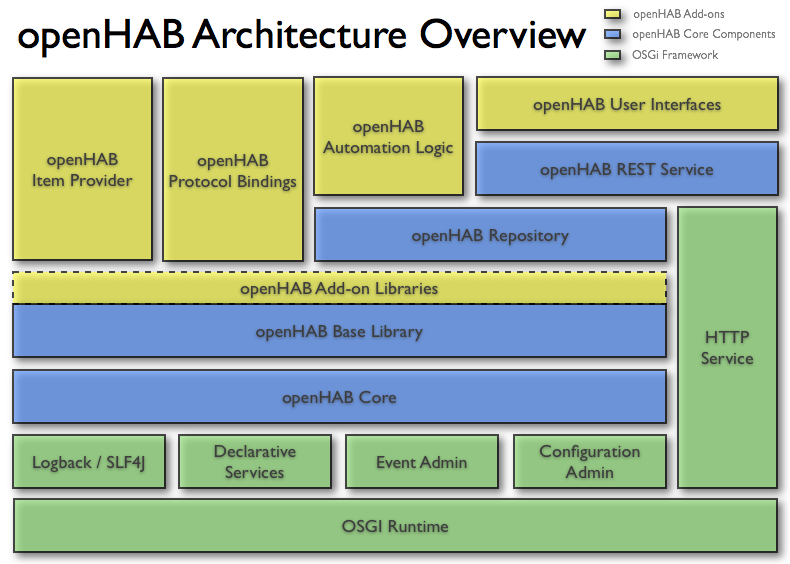
\includegraphics[width=15cm,height=10cm,keepaspectratio]{images/openhab-architecture.png}
        \caption{Architektur der openHAB Plattform \cite{openHAB-architecture2013}}
        \label{fig:architectureopenHAB}
    \end{figure}
    \\
    %\pagebreak
    \linebreak
    Mit der wesentlichen Aktualisierung von \acs{OPENHAB} zur architektonisch aktuellen Version \acs{OPENHAB} 2.0 gab es auch einige Änderungen an dem 
    grundlegenden Aufbau des Systems. Es basiert hauptsächlich auf dem Eclipse SmartHome Framework und nutzt Apache Karaf zusammen mit 
    Eclipse Equinox, um eine \acs{OSGI} Laufzeitumgebung zu erstellen. Jetty wird als \acs{HTTP} Server verwendet. 
    \\
    \linebreak
    \textit{Eclipse SmartHome}\footnote{Eclipse SmartHome. \url{https://projects.eclipse.org/projects/iot.smarthome} Abgerufen am 29.04.2022} 
    ist ein \acs{IoT} Projekt, welches sich aus der ersten Version der \acs{OPENHAB} Plattform entwickelte. 
    Diese wurde von der Eclipse Foundation übernommen und weiterentwickelt. Es stellt das Kern-Framework für Smart Home Systeme dar 
    und ist essentieller Bestandteil der \acs{OPENHAB} Plattform. Das Framework ist mittlerweile archiviert und erhält keine weiteren 
    Aktualisierungen.
    \\
    \linebreak
    \textit{Apache Karaf}\footnote{Apache Karaf. \url{https://karaf.apache.org/} Abgerufen am 29.04.2022} 
    ist eine \acs{OSGI} basierte Laufzeitumgebung, über die verschiedene Komponenten mittels Container 
    bereitgestellt werden können. Dieses Framework zählt zu denen der Apache Software Foundation und unterliegt der Apache V2 Lizenz.
    \\
    \linebreak
    \textit{Eclipse Equinox}\footnote{Eclipse Equinox. \url{https://www.eclipse.org/equinox/} Abgerufen am 29.04.2022} ist eine modulare 
    Java basierte Laufzeitumgebung und eine Implementierung des \acs{OSGI} Frameworks. Der Begriff der \textit{Bundles} ist das 
    Kernstück der \acs{OSGI}-Spezifikation. Diese werden verwendet, um die Modularität für Java zu erfassen. Ein Bundle ist 
    eine Standard-Java-JAR-Datei, dessen Manifest zusätzliches Markup enthält, welches das Bundle identifiziert und seine Abhängigkeiten 
    angibt. Als solches ist jedes Bundle vollständig selbstbeschreibend \cite{openHAB-article}. 
    \begin{figure}[hbt!]
        \centering
        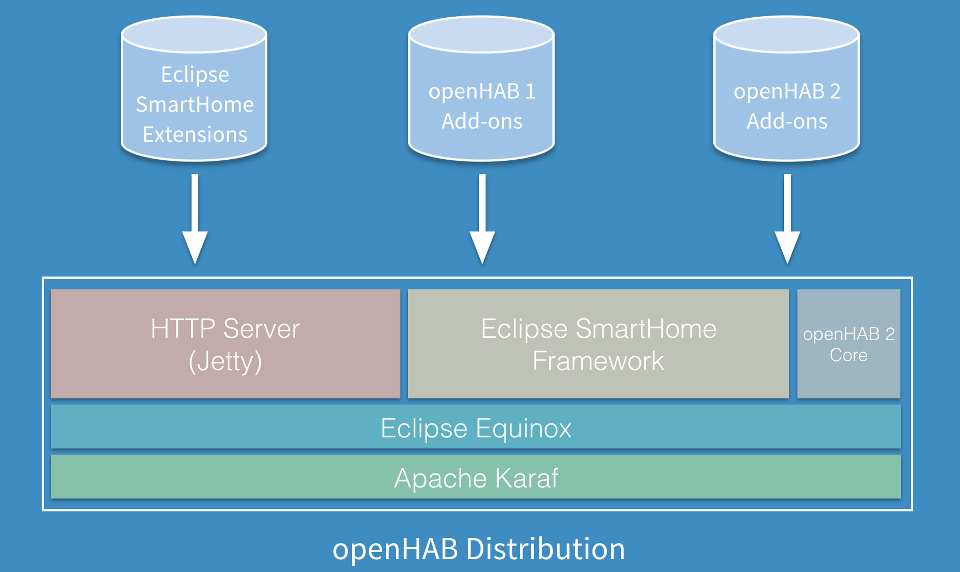
\includegraphics[width=15cm,height=9cm,keepaspectratio]{images/openhab-2-architecture.png}
        \caption{Architektur der openHAB 2.0 Plattform \cite{kaikreutzer2016}}
        \label{fig:architectureopenHAB2}
    \end{figure}
    \\
    %\pagebreak
    %\linebreak
    Die Plattform befindet sich aktuell in der Version 3. Grundlegende Änderungen der Architektur gab es jedoch bei der Aktualisierung 
    der Systemversion von zwei auf drei nicht, weshalb obiges Architekturschaubild (\ref{fig:architectureopenHAB2}) als aktuelles gilt. 
    Die Änderungen beinhalteten Erweiterungen des Systems, die für den Nutzer sichtbar waren, und zusätzlich Maßnahmen, um veraltete 
    Funktionen und Konzepte abzuschalten sowie Refactorings, um die grundlegende Architektur zu vereinfachen, jedoch nicht zu ändern. 
    Die Dokumentation\footnote{Aktualsisierung von openHAB 2 zu 3. \url{https://github.com/openhab/openhab-distro/wiki/Breaking-Changes-in-openHAB-3/139901f0ef7ee8b5b7dd480204ddf5069f030f50} Abgerufen am 03.07.2022} 
    zu Änderungen und Versionsupdates ist der Organisation auf GitHub zu entnehmen.
    \\
    \linebreak
    Der Open-Source-Standard \textit{OSGi} beschreibt einen Ansatz zur Modularisierung von Software. Die Verwendung des 
    Frameworks setzt ebenso eine \ac{JVM} voraus. 
    Die \acl{JVM}\footnote{Beschreibung der JVM. \url{https://www.javatpoint.com/jvm-java-virtual-machine} Besucht am 01.05.2022} 
    ist der Teil der Java-Laufzeitumgebung, die für die Ausführung des Java-Bytecodes verantwortlich ist.
    \\
    Die im Kontext des \acs{OSGI} betitelten \textit{Bundles} sind einzelne Module und bilden die kleinste Einheit der Modularisierung. Aus technischer Sicht ist 
    das Konstrukt eine \ac{JAR}-Datei mit Metainformationen. Diese sind in einer Manifestdatei gespeichert. Durch die eindeutige 
    Identifizierung von \textit{Bundles} ist es in \acs{OSGI} möglich, sie mit demselben Namen, jedoch unterschiedlicher 
    Versionen gleichzeitig zu nutzen und auszuführen \cite{openHAB-article}. 
    \begin{figure}[hbt!]
        \centering
        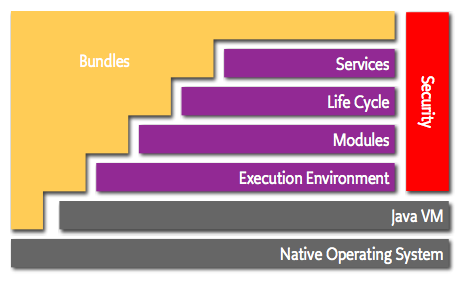
\includegraphics[width=10cm,height=9cm,keepaspectratio]{images/osgi-architecture.png}
        \caption{OSGi Schichtenarchitektur \cite{openhab-osgi}}
        \label{fig:osgilayer}
    \end{figure}
    \\
    %\pagebreak
    %\linebreak
    Weitere Details der \acs{OSGI}-Architektur\footnote{Erläuterung von OSGi. \url{https://www.openhab.org/docs/developer/osgi/osgi.html} Besucht am 01.05.2022} 
    sind der \acs{OPENHAB} Dokumentation zu entnehmen.

\subsection{Ziele und Schwerpunkte} 
    \begin{quote}
        „openHAB empowering the smart home\footnote{Log und Label von openHAB \url{https://www.openhab.org/} Besucht am 01.05.2022}“
    \end{quote}
    Das Ziel, das mit der openHAB Anwendung verfolgt wird, ist allgemein die zentrale Steuerung von Geräten innerhalb eines 
    Wohnraumes.
    \begin{quote}
        „... is an open source, technology agnostic home automation platform which runs as the center of your smart home!\footnote{Übersicht der openHAB Dokumentation. \url{https://www.openhab.org/docs/} Besucht am 01.05.2022}“
    \end{quote}
    
\subsection{Stärken und Schwächen}
    Die Stärken, die \acs{OPENHAB} mit sich bringt, werden schon in den Dokumentationen der Plattform aufgegriffen und bei der Nutzung der Anwendung 
    schnell deutlich. Mit der Plattform können eine Vielzahl von Geräten und Systemen integriert werden, die miteinander 
    kommunizieren. In der einzigen von \acs{OPENHAB} gegebenen Lösung können Heimautomatisierungssysteme, intelligente Geräte und 
    andere Technologien, darunter beispielsweise Kommunikationsprotokolle, integriert werden \cite{openhab-strength}. Durch die in 
    dem letzten großen Update der Plattform hinzukommende einheitliche Benutzeroberfläche, die die Bedienung von Geräten und 
    Systemen vereinfacht, ist die Integration von neuen Geräten einfacher. Mit dem Ansatz von 
    Automatisierungsregeln können alle Geräte bei Bedarf miteinander kommunizieren. Das Aufstellen von solchen Regeln ist 
    herstellerunabhängig und macht die Automatisierung flexibler. Der dritte und letzte Punkt der Stärken ist die allgemeine 
    Vielfältigkeit und Flexibilität der Plattform. Hiermit ist im Allgemeinen die Umsetzung von Use Cases und Automatisierungen 
    gemeint.
    \\
    \linebreak
    Zu den Schwächen zählt hauptsächlich die vielschichtige und weitgestrickte Architektur.
    Das System an sich 
    und der Umgang damit stellt sich als komplex dar. Das Aufsetzen der Plattform und das Verstehen der Konzepte und  
    Möglichkeiten sind sehr zeitintensiv. Dies spiegelt die Dokumentation der Software wieder \cite{openhab-strength}. 
    \\
    Eine zusätzliche Schwäche ist die Weiterentwicklung des Systems. Diese findet langsam und nicht konstant statt. Auslöser 
    dafür ist die Architektur und deren Abhängigkeiten zu weiteren Frameworks und Bibliotheken. Auch nimmt der Prozess bis zur 
    Genehmigung von Weiterentwicklungen viel Zeit in Anspruch. Dies ist möglicherweise mit ein Grund, weshalb neue Versionen und 
    Updates nur unregelmäßig zu beobachten sind. 

    \subsection{Optionen der Regel- und Automatisierungserstellung}
        %Skizzierung der Möglichkeiten des Tools
        Im Vergleich zu Home Assistant bietet \acs{OPENHAB} zur Definition und Erstellung von Regeln mehrere Möglichkeiten an, die über deren Oberfläche definiert werden können. 
        Die Konfiguration solcher Regeln kann jedoch mit unterschiedlichen Methoden umgesetzt werden. Zum 
        einen mit einem visualisierten Baukasten Werkzeug Namens \textit{Blockly}\footnote{Ein visueller Code Editor von Google. \url{https://developers.google.com/blockly} Besucht am 29.05.2022} 
        und zum anderen über eine \ac{DSL}, im Deutschen eine domänenspezifische Sprache\footnote{Erklärung der domänenspezifischen Sprache. \url{https://martinfowler.com/dsl.html} Besucht am 29.05.2022}. 
        \acs{OPENHAB} verwendet für die Syntax der Regeldefinition Xbase\footnote{Erläuterung des Xbase Frameworks. \url{https://www.eclipse.org/Xtext/index.html} Besucht am 29.05.2022} 
        und darauf aufbauend Xtend\footnote{Spezieller Javadialekt. \url{https://www.eclipse.org/xtend/index.html} Besucht am 29.05.2022}. 
        Diese \acs{DSL} gibt ein Konstrukt vor, mit dem Regeln definiert werden können. Dies sieht wie folgt aus:
        \\
        %\linebreak 
        \begin{lstlisting}[language=Java, frame=lines, xleftmargin=\parindent, style=algoBericht, label={code:Xbase}, captionpos=b, caption={Konstrukt zur Regeldefinition über Xbase}]
        rule "<RULE_NAME>"
        when
            <TRIGGER_CONDITION> [or <TRIGGER_CONDITION2> [or ...]]            
        then
            <SCRIPT_BLOCK>
        end
        \end{lstlisting}
        Jede Regel bekommt einen eindeutigen Namen. Danach muss eine Bedingung implementiert werden, bei deren Eintreffen 
        eine bestimmte, beliebige Aktion ausgelöst wird. Die Logik der Regel wird über den Skript-Block eingesetzt. Für die Syntax 
        der Regellogik wird \textit{Xtend} verwendet. 

\section{Vergleich von Home Assistant und openHAB}
\label{sec:comparison-HAOS-openHAB}
    %Allgemein gültiger Vergleich (Aufbau, Architektur, Schwerpunkte (Fokus), Umsetzungen, Konnektivität, etc.)
    % https://everythingsmarthome.co.uk/home-assistant-vs-openhab-which-one-is-better/
    % https://smarthome.msuttner.de/openhab-2/vergleich-openhab-vs-home-assistant/ 
    % https://www.electronicshub.org/openhab-vs-home-assistant/ 
    % https://smarthome.university/your-smart-home-platform-home-assistant-vs-openhab/ 
    % https://purdylounge.com/openhab-vs-home-assistant/ 
    Nach der Erläuterung der beiden Softwarelösungen im Bereich der Smart Home Plattformen werden diese abschließend 
    gegenübergestellt, um weitere Aspekte miteinander zu vergleichen. Grundlage dafür sind persönliche Erfahrungen, als auch 
    Eindrücke von Nutzern und Experten. Die Tabellen (\ref{tab:comparisonTableHAOS-openHAB-part1} \& \ref{tab:comparisonTableHAOS-openHAB-part2}) zum Vergleich 
    der Plattformen ist dem Anhang (\ref{appendix:comparison}) zu entnehmen.
    \\
    \linebreak
    Zusammenfassend zu dieser tabellarischen Gegenüberstellung ist zu sagen, dass beide Plattformen Vorzüge aufweisen.  
    Beide Ansätze bieten eine gute Grundlage, die Automatisierungen in dem eigenen Gebäude voranzutreiben. Die Entscheidung, welches 
    Tool verwendet werden soll, liegt in der Verantwortung des Nutzers. Übergreifend sind die beiden Open-Source-Lösungen eine gute 
    Alternative zu kommerziellen Produkten und Lösungen, sofern der Nutzer herstellerunabhängig interagieren möchte. Dennoch ist 
    es für Nutzer und Entwickler mit einem hohen Aufwand verbunden, Automationen und Regeln zu definieren, da Werkzeuge eingesetzt werden, 
    die nicht dem Standard der verwendeten Programmiersprache, beispielsweise von Java, 
    entsprechen. Dadurch muss zuerst die Funktionsweise des Frameworks verstanden werden, um anschließend Automationen und 
    Regeln definieren und anwenden zu können. Beide Lösungen versuchen diese Herausforderung anzugehen, indem über eine Weboberfläche 
    die Regeln konfiguriert und erstellt werden können. Home Assistant nutzt hierfür, wie bereits erläutert, das YAML-Dateiformat. Im 
    Gegenzug dazu verwendet \acs{OPENHAB} ein Framework, das das Konstrukt der Regeldefinition starr vorgibt. Alternativ können Regeln auch 
    mittels \textit{Blockly} realisiert werden. 
    \\
    Beide Softwarelösungen bieten einen unterschiedlichen Ansatz zur Regeldefinition, jedoch ist die Flexibilität 
    auf integrierte Komponenten beschränkt. Das bedeutet, dass nur vom System abbildbare Komponenten, 
    Integrationen und Verknüpfungen verwendet werden können. Gibt es beispielsweise für eine Komponente oder ein Gerät keine 
    Integration oder kein Add-on, so muss dieses erst im Quellcode als Packet implementiert und angeboten werden, bevor der 
    Anwender dieses benutzen kann. 
    \\
    \linebreak
    Die soeben erläuterten Grundlagen geben einen Einblick in eine Domäne des \acs{IoT}. Mit den Kommunikationsprotokollen werden Standards 
    und derzeit oft verwendete Technologien beschrieben. Das \acs{MQTT}-Protokoll wird im Rahmen dieser Arbeit von Anfang an verwendet. 
    Die Erläuterung von zwei Softwareplattformen gibt einen Überblick 
    darüber, welche Lösungen bereits vorhanden sind und wie sich deren Aufbau gestaltet. Diese Information ist notwendig, um im 
    weiteren Verlauf die Konzeption als auch die anschließende Analyse nachvollziehen zu können.

 